\section{The \instname\ data reduction flow.}
\label{sec:reduction_flow}


The overall data flow of the \instname\ pipeline is displayed in Figure \ref{fig:reduction_cascade}.

 
\begin{figure}[h!]
\centering

\includegraphics[width=0.9\textwidth]{../instrument_tutorial/figures/reduction_cascade.jpg}
\caption{The data reduction cascade of the \instname\ workflow.}
\label{fig:reduction_cascade}
\end{figure}



The reduction cascade is organized in tasks, which represent
well-defined steps in the process. Tasks can be grouped inside
sub-workflows.  Each task runs a recipe; the detailed description of
the algorithms, input, outputs and recipe parameters used in each
recipe are available in the pipeline manual. Here, we present only the
description of most important features.

The \wkfname\  \edps\ workflow is designed to execute the tasks that
deliver the final reduced data cube for each dataset. It can be either
the product of a single exposure, or the combination of multiple
exposures. Only calibrations needed by the selected the scientific
exposures are processed.

It is possible to set \edps\ to perform the data reduction until a
certain step of the reduction chain (e.g. to reduce only standar
stars, or only flat fields).  This is done by specifying the desired
tasks in the field {\bf Select reduction target} of the {\bf Raw Data}
tab.

The reduction steps of the \wkfname\ workflow are listed below. Before
starting the reduction, the parameters of the recipes associated to
each task can be configured by pressing the button

\includegraphics[width=0.8cm]{../common/figures/configure_dataset.jpg}
close to each dataset configuration.
See for more info on the configuration editor \ref{sec:configuration_editor}



\subsection{Bias subtraction}
The task {\bf bias} reduces raw bias frames to generate a combined masterbias. It
runs the recipe {\bf muse\_bias}.

\subsection{Computation of dark current}
The task {\bf dark} runs the recipe {\bf muse\_dark}. If raw dark
frames are present, the actor processes them and creates a master
dark. This product is currently used only for instrument monitoring
but not for scientific reduction. Dark frames are taken monthly,
therefore they might not represent the dark current at the time of the
observations, and they add noise to the final products. If needed,
darks can be used in the reduction cascade by setting the workflow
parameter {\bf use\_darks} to "yes" in the {\bf science\_parameters}
parameter set.

\subsection{Flat field correction}
The task {\bf lamp\_flat} runs the recipe {\bf muse\_flat}. It processes the raw flat-fields
exposures, producing a master flat and a trace table.

\subsection{Wavelength correction}
The task {\bf arc} executes the recipe {\bf muse\_wavecal}. It processes the raw arc frames,
producing a table with the wavelength solution.

\subsection{Characterization of the line spread function}

This subworkflow is designed to run the recipe {\bf muse\_lsf}
to produce a calibration that characterize the line spread function.
In \instname, the generation of the line spread function can be done by
processing raw arc frames (done by the task
{\bf line\_spread\_function\_arc}) or by dedicated calibrations (done by the
task {\bf line\_spread\_function\_lsf}). Alternatively, a static calibration
is used. The behavior is determined by the workflow parameter
{\bf lsfmode}, which is described in Section \ref{sec:configuration_lsf}.






\subsection{Monitoring calibrations, geometry and astrometry calibrations}

The subworkflow {\bf monitoring\_and\_long\_term\_calibs} contains
tasks aimed at creating long term calibrations, such as geometry
calibrations (task {\bf geometry}, recipe {\bf muse\_geometry}),
astrometric calibrations (tasks {\bf preprocess\_astrometry}, {\bf
  astrometry}, recipes {\bf muse\_scibasic}, {\bf
  muse\_astrometry}). These calibrations are distributed by the ESO
archive together with the scientific data. It is anyway possible to
recreate these calibrations from raw data by setting the workflow
parameters {\bf recompute\_geometry} and {\bf recompute\_astrometry}
to "yes".

Additionally, the subworkflow contains tasks aimed at monitoring the
instrument performance such as the throughput (task throughput, recipe
{\bf muse\_ampl}), the instrument linearity and gain (task {\bf
  linearity\_and\_gain}, recipe {\bf muse\_lingain}). These tasks
however, are executed only at the observatory, and they are not used
in the data reduction flow.

\subsection{Sky subtraction}

The subworkflow {\bf Process and combine sky} contains the tasks in charge of evaluating the sky background from dedicated
sky exposures.

They are:
\begin{itemize}
\item {\bf preprocess\_sky}. It runs the recipe {\bf muse\_scibasic} on dedicated sky exposures.
\item {\bf sky}. It runs the recipe {\bf muse\_create\_sky} to generate SKY\_LINES and SKY\_CONTINUUM calibrations.
\end{itemize}

Sky subtraction can also be done by evaluating the sky contribution
directly on regions in the target field of view that is free from
contamination from astronomical sources.  The most important products
to check, regardless of the method used, are the

\begin{itemize}
\item SKY\_CONTINUUM. It should not contain features that are typical of astronomical objects. 
For example, if the sky region contains HII regions, the Halpha emission lines are not registered as a sky line in the 
input list of sky lines. As a consequence, it will be present in the SKY\_CONTINUUM and therefore subtracted from the 
target spectrum.
\item SKY\_MASK. A comparison between the image field of view and the sky mask should confirm that astronomical sources are not included as sky regions.

\end{itemize}

If the SKY\_MASK overlap with some source or if SKY\_CONTINUUM contains astrophysical signal such as nebular emission lines, 
consider to decrease the recipe parameter {\bf skymodel-fraction} or to provide a custom SKY\_MASK in the input directory.

SKY\_CONTINUUM and SKY\_MASK products are available from the tasks sky (if dedicated sky observations are used) and 
object (if the sky was evaluated on the target field of view). Click on the magnifying glass
symbol close to the appropriate task, and select the tab {\bf Output Files}. Products can be inspected via the {\tt fv} fits 
viewer (if available).

More information on the sky background removal are given
in Section \ref{sec:configuration_sky_subtraction}.



This subworkflow contains also the tasks that consider dedicated sky exposures as self-contained science exposures and
processes and combine them as such
(tasks {\bf preoprocess\_sky\_sky}, {\bf object\_sky}, {\bf alignment\_sky}, and {\bf combine\_sky}).
The strategy to combine sky exposures is the same as for the regular science exposures.

\subsection{Flux calibration}

The subworkflow {\bf response} contains the tasks to process standard stars and create the response and telluric
corrections. They are:

\begin{itemize}
\item {\bf preprocess\_standard}. It runs the recipe {\bf muse\_scibasic} on raw standard stars

 \item {\bf response}. It runs the recipe {\bf muse\_standard} and
   generate STD\_RESPONSE and STD\_TELLURIC calibrations. To disable
   telluric correction on your data, set the workflow parameter {\bf
     telluric\_correction} to 'FALSE', see Section
   \ref{sec:configuration_telluric_correction}.

\end{itemize}

\subsection{Reduction and combination of scientific exposures}

The subworkflow {\bf Process and combine object} contains the tasks in
charge of aligning and combining scientific exposures. They are:

\begin{itemize}
\item {\bf preprocess\_science}. This task runs the recipe {\bf muse\_scibasic} on scientific exposures.
\item {\bf autocalibration\_from\_object\_sky}. This tasks select autocalibration coefficients computed from sky exposures, if
  requested. It is not directly associated to any recipe, see Section \ref{sec:configuration_autocalibration}.

\item {\bf object}. This task runs the recipe {\bf muse\_scipost} to reduce a single scientific exposure.
\item {\bf source\_detection}. This task runs the recipe {\bf
  muse\_detection} to detect sources in the datacube of each
  individual exposure and create a source catalog. The source catalogs
  are used for the alignment of the exposures.
\item {\bf alignment}. This tasks runs the recipe {\bf muse\_alignment} to correct for coordinate offsets the exposures that are meant
  to be combined together.
  It uses sources detected in the previous step to compute the offsets.
\item  {\bf object\_combination}. This tasks runs the recipe {\bf muse\_exp\_combine} and combines individual exposures to produce the
  final datacube (see Section \ref{sec:configuration_combination} on how to specify exposures to be combined).

\end{itemize}

The most important thing to check in this step is whether or not the
images to combine were properly aligned.  In the Reduction Queue tab,
locate and expand the reduced dataset you want to check, and click on
the magnifying glass symbol close to the alignment task as shown in
Figure \ref{fig:alignment_1}.

\begin{figure}[h!]
\centering
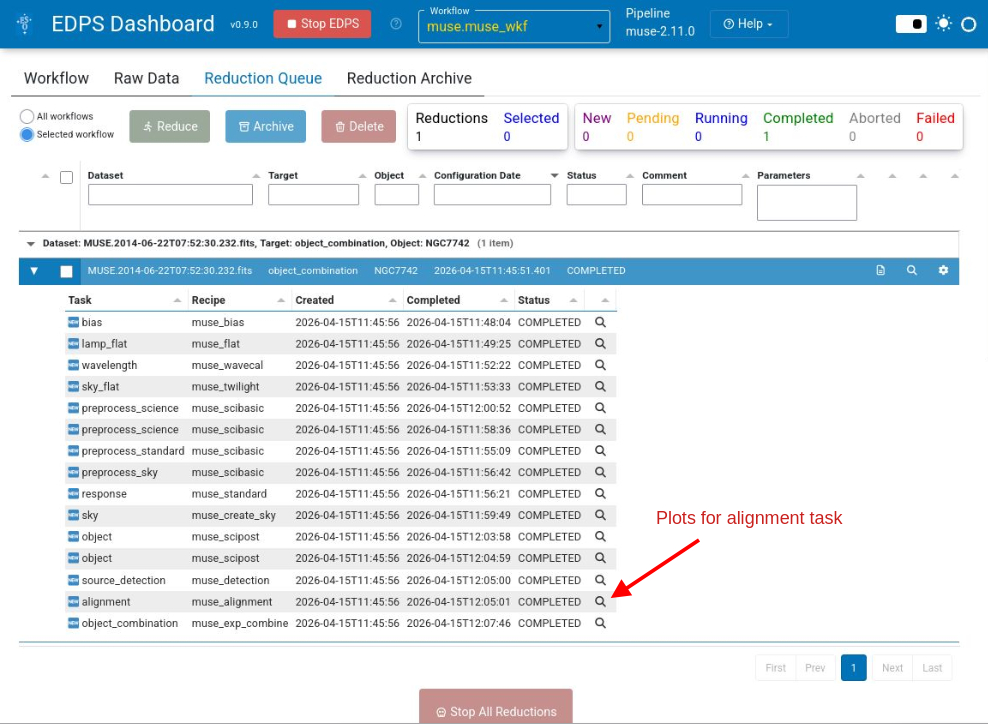
\includegraphics[width=0.9\textwidth]{../instrument_tutorial/figures/alignment_1.jpg}
\caption{How to display the quality plots for the alignment task.}
\label{fig:alignment_1}
\end{figure}

The following interactive plot will appear, showing the preview of the
combination of the field of views after alignment correction (Figure
\ref{fig:alignment_2}). In the case of good alignment, there are no
duplicated sources.

\begin{figure}[h!]
\centering
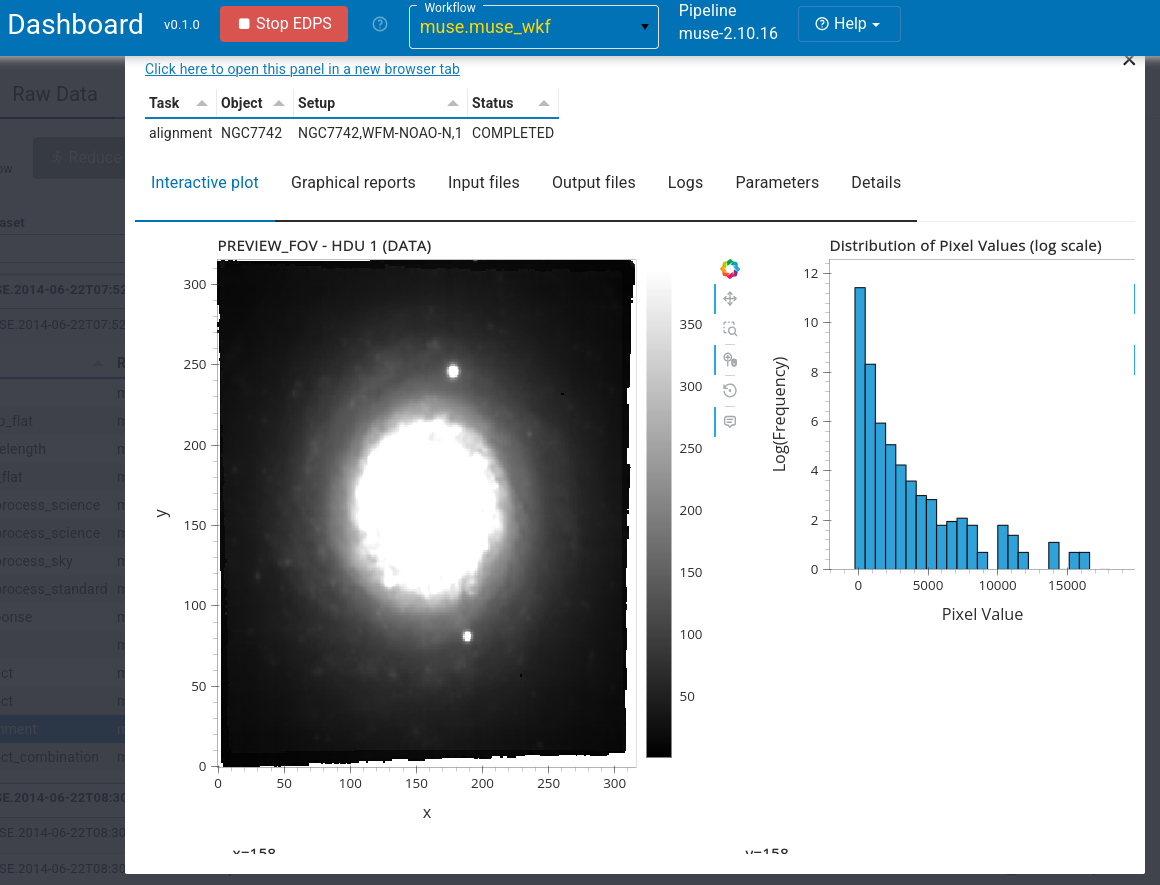
\includegraphics[width=0.9\textwidth]{../instrument_tutorial/figures/alignment_2.jpg}
\caption{Quality plots for the alignment. On the left, the overview of
  the combined field of view after alignment, on the right an
  histogram of the pixel counts. Other information such as the list of
  inputs and outputs, recipe logs, recipe parameters, and job
  technical info can be accessed from the various tabs.}
\label{fig:alignment_2}
\end{figure}

In case of bad alignment, here we provide some tipps that can help in
improving the alignment.  Re-configure the reduction of the dataset by
pressing the 
\includegraphics[width=0.8cm]{../common/figures/configure_dataset.jpg} button and
set the recipe parameter accordingly in the configuration window
(Sect. \ref{sec:configuration_editor}).



\begin{itemize}
\item {\bf Task source\_detection}.

  \begin{itemize}

  \item In the case of too many or too few detected sources (e.g. in
    crowded fields), decrease or increase the parameters {\bf
      source\_min} and {\bf source\_max} (minimum and maximum number
    of detections, respectively). Sometimes it helps to change the
    initial threshold level, via the parameter {\bf
      start\_threshold\_sigma}. To prevent the threshold to go too low
    during iterations, one can set the minimum accepted threshold via
    the parameter {\bf threshold\_limit}.

  \item A lot of sources are detected in the edges of the field of
    view. This can be solved by increasing the parameter {\bf
      border\_distance\_pxl}.

  \end{itemize}
  
    \item {\bf Task alignment}.

      \begin{itemize}
      
  \item The maximum number of allowed stars is detected, but the
    alignment is not correct. This can happen in crowded fields, and
    the alignment algorithm does not find the correct matching between
    the sources detected in different frames. There are two tricks to
    overcome this issue. First, one could either decrease the number
    of maximum sources allowed in the detection. However, this
    solution is not advisable for mosaicing, because the number of
    reference sources in the overlapping regions could be too
    small. Second, if the offsets are known to be small, the user can
    decrease value of the first search radius and set the
    corresponding recipe parameter ({\bf search\_radii}) to, for
    example, '10.,4.,2.,0.8'. The first entry (10 in this example)
    forces the matching algorithm to find offsets of at most 10
    arcseconds.
    
  \item Avoid source misidentification across exposures. To avoid to
    associate the wrong sources, one can specify the maximum
    difference in magnitude or in fwhm between sources in different
    exposures. This can be done by setting the recipe parameters {\bf
      threshold\_on\_mag} and {\bf threshold\_on\_fwhm}, respectively.

      \end{itemize}
      
\end{itemize}

Tipp: In case of complicated alignment, it might be advisable to
specify {\bf alignment} as reduction target when creating the datasets
in the {\bf Raw Data} tab. In this way the reduction stops at this
step, without wasting resources to combine the exposures. After the
correct recipe parameters set has been found, the full reduction
cascade can be triggered.


